\documentclass[12pt,a4paper]{article}
%%%%%%%%%%%%%%%%%%%%%%%%%%%%%%%%%%%%%%%%%%%%%%%%%%%%%%%%%%%%%%%%%%%%%%%%%%%%%%%%
%%%%%%%%%%%%%%%%%%%%%%%%%%%%%%%%%%%%%%%%%%%%%%%%%%%%%%%%%%%%%%%%%%%%%%%%%%%%%%%%
%%% Template for AIMS Rwanda Assignments         %%%              %%%
%%% Author:   AIMS Rwanda tutors                             %%%   ###        %%%
%%% Email: tutors2017-18@aims.ac.rw                               %%%   ###        %%%
%%% Copyright: This template was designed to be used for    %%% #######      %%%
%%% the assignments at AIMS Rwanda during the academic year %%%   ###        %%%
%%% 2017-2018.                                              %%%   #########  %%%
%%% You are free to alter any part of this document for     %%%   ###   ###  %%%
%%% yourself and for distribution.                          %%%   ###   ###  %%%
%%%                                                         %%%              %%%
%%%%%%%%%%%%%%%%%%%%%%%%%%%%%%%%%%%%%%%%%%%%%%%%%%%%%%%%%%%%%%%%%%%%%%%%%%%%%%%%
%%%%%%%%%%%%%%%%%%%%%%%%%%%%%%%%%%%%%%%%%%%%%%%%%%%%%%%%%%%%%%%%%%%%%%%%%%%%%%%%


%%%%%% Ensure that you do not write the questions before each of the solutions because it is not necessary. %%%%%% 


%%%%%%%%%%%%%%%%%%%%%%%%% packages %%%%%%%%%%%%%%%%%%%%%%%%
\usepackage{amsmath}
\usepackage{amssymb}
\usepackage{placeins}
\usepackage{amsthm}
\usepackage{amsfonts}
\usepackage{graphicx}
\usepackage[all]{xy}
\usepackage{tikz}
\usepackage{verbatim}
\usepackage{float}
\usepackage{bbm} %indicator function 1 package
\usepackage{bbold} %indicator function 1 package with bold
\usepackage[left=2cm,right=2cm,top=3cm,bottom=2.5cm]{geometry}
\usepackage{hyperref}
\usepackage{caption}
\usepackage{subcaption}
\usepackage{psfrag}
\usepackage{mathrsfs}

%%%%%%%%%%%%%%%%%%%%% students data %%%%%%%%%%%%%%%%%%%%%%%%
\newcommand{\student}{Yusuf Brima}
\newcommand{\course}{Statistical Machine Learning for Data Science}
\newcommand{\assignment}{2}

%%%%%%%%%%%%%%%%%%% using theorem style %%%%%%%%%%%%%%%%%%%%
\newtheorem{thm}{Theorem}
\newtheorem{lem}[thm]{Lemma}
\newtheorem{defn}[thm]{Definition}
\newtheorem{exa}[thm]{Example}
\newtheorem{rem}[thm]{Remark}
\newtheorem{coro}[thm]{Corollary}
\newtheorem{quest}{Question}[section]

%%%%%%%%%%%%%%  Shortcut for usual set of numbers  %%%%%%%%%%%

\newcommand{\N}{\mathbb{N}}
\newcommand{\Z}{\mathbb{Z}}
\newcommand{\Q}{\mathbb{Q}}
\newcommand{\R}{\mathbb{R}}
\newcommand{\C}{\mathbb{C}}

%%%%%%%%%%%%%%%%%%%%%%%%%%%%%%%%%%%%%%%%%%%%%%%%%%%%%%%555
\begin{document}

%%%%%%%%%%%%%%%%%%%%%%% title page %%%%%%%%%%%%%%%%%%%%%%%%%%
\thispagestyle{empty}
%\begin{figure}
%    \centering
%    \includegraphics[width=\textwidth]{aims_rwanda.jpg}
%\end{figure}
\begin{center}
\textbf{AFRICAN INSTITUTE FOR MATHEMATICAL SCIENCES \\[0.5cm]
(AIMS RWANDA, KIGALI)}
\vspace{1.0cm}
\end{center}

%%%%%%%%%%%%%%%%%%%%% assignment information %%%%%%%%%%%%%%%%
\noindent
\rule{17cm}{0.2cm}\\[0.3cm]
Name: \student \hfill Assignment Number: \assignment\\[0.1cm]
Course: \course \hfill Date: \today\\
\rule{17cm}{0.05cm}
\vspace{1.0cm}
\section*{Exercise 1}
\begin{enumerate}
	\item[(1)] 
			The empirical  Probability of Correct Classification  on the test set $\widehat{\text{PCC}}_{te}$ of the learning machine $\widehat{f} $  is thus: 
			\begin{align*}
					\widehat{\text{PCC}}_{te}(\widehat{f})  &=  \frac{\widehat{\text{TPR}}(\widehat{f}) + \widehat{\text{ TNR}}(\widehat{f}) }{2}\\
			\end{align*}
			
			Where 
			\begin{align*}
						\widehat{\text{TPR}}(\widehat{f}) &=  \frac{\widehat{ \text{TP} }(\widehat{f}) }{  \widehat{ \text{TP} }(\widehat{f})  + \widehat{ \text{FN} }(\widehat{f})  }\\
								&= \frac{7}{8}
			\end{align*}
And 
			\begin{align*}
						\widehat{\text{TNR}}(\widehat{f})  &=  \frac{\widehat{ \text{TN} }(\widehat{f}) }{  \widehat{ \text{TN} }(\widehat{f})  + \widehat{ \text{FP} }(\widehat{f})  }\\
								&= \frac{7}{8}
			\end{align*}
Therefore
			\begin{align*}
					\widehat{\text{PCC}}_{te}(\widehat{f})  &= \frac{\frac{7}{8} + \frac{7}{8} }{2}\\
					&= 0.875\\
			\end{align*}
	
Whilst the theoretical/ideal  Probability of Correct Classification  on the test set $\text{PCC}_{te}$ of the learning machine $\widehat{f} $  is thus: 
			\begin{align*}
					\text{PCC}_{te}(\widehat{f})  &=  \frac{\text{TPR}(\widehat{f}) + \text{ TNR}(\widehat{f}) }{2}\\
			\end{align*}
			
	\item[(2)] $\widehat{\text{R}}_{te}(\widehat{f})$ is the empirical Risk Functional on the test set $\mathscr{D}_{te}$ for the learning function  $\widehat{f}$. 
			\begin{align*}
						\widehat{\text{R}}_{te}(\widehat{f})  &= \frac{ \widehat{ \text{FN} }(\widehat{f}) + \widehat{ \text{FP} }(\widehat{f})  }{  \widehat{ \text{FN} }(\widehat{f}) + \widehat{ \text{FP} }(\widehat{f})  + \widehat{ \text{TN} }(\widehat{f}) + \widehat{ \text{TP} }(\widehat{f})  }\\
						&= \frac{2}{16}
			\end{align*}
Whilst the true/theoretical Risk Functional $\text{R}_{te}(\widehat{f})$ on  the test set $\mathscr{D}_{te}$ for the learning function  $\widehat{f}$ is thus:
			\begin{align*}
						\text{R}_{te}(\widehat{f})  &=  \frac{ \text{FN} (\widehat{f}) + \text{FP} (\widehat{f})  }{  \text{FN} (\widehat{f}) + \text{FP} (\widehat{f})  +  \text{TN} (\widehat{f}) + \text{TP} (\widehat{f})  }\\
			\end{align*}
	\item[(3)] 	$\widehat{M}_{te} $, the confusing matrix of $\widehat{f}$ \vspace{0.7cm} \\
             \vspace{1.2cm}
            $\text{y}$
				\begin{tabular}{|l|l|l|}
					\hline
 					& -1 & +1 \\ \hline
				-1 & 7 & 1 \\ \hline
				+1 & 1 & 7 \\ \hline
				\end{tabular}
	
		
	\item[(4)] 
			\begin{align*}
						\frac{\text{trace}(\widehat{M}_{te} ) }{|\text{D}_{te} |} &= \frac{  \widehat{ \text{TN} }(\widehat{f}) + \widehat{ \text{TP} }(\widehat{f})   }{ |\text{D}_{te} |}\\
						&=  \widehat{A}(\widehat{f})  =  \frac{14}{16} 
			\end{align*}
			This indicates the proportion of correctly classified positive (+1) test set data, in this case, the learning machine correctly classified $87.5\%$ of the test set correctly.
		\item[(5)] The True Positive Rate  is a measure of the ratio of True Positives over the Positive Ground Truth. In other words  $\mathbb{P} (f(\text{x}_i) = 1 | \text{y}_i = 1)$ .The empirical True Positive Rate $\widehat{\text{TPR}}(\widehat{f}) $ of the learning function  on $\mathscr{D}_{te} $ is defined below : 
					\begin{align*}
						\widehat{\text{TPR}}(\widehat{f}) &=  \frac{\widehat{ \text{TP} }(\widehat{f}) }{  \widehat{ \text{TP} }(\widehat{f})  + \widehat{ \text{FN} }(\widehat{f})  }\\
								&= \frac{7}{8}
			\end{align*}
		And the  theoretical/ideal True Positive Rate $\text{TPR}(\widehat{f}) $ of the learning function  on $\mathscr{D}_{te} $ is thus: 
		\begin{align*}
						\text{TPR}(\widehat{f}) &=  \frac{\text{TP} (\widehat{f}) }{  \text{TP} (\widehat{f})  + \text{FN} (\widehat{f})  }\\
			\end{align*}
	\item[(6)] This indicates the proportion of incorrectly classified  negative (-1) test set data, in this case, the learning machine correctly classified $12.5\%$  negative (-1) of the test set incorrectly.
		\item[(5)] The False Positive Rate  is a measure of the ratio of False Positives over the Positive Ground Truth.  In other words  $\mathbb{P} (f(\text{x}_i) = 1 | \text{y}_i = -1)$ .The empirical True Positive Rate $\widehat{\text{TPR}}(\widehat{f}) $ of the learning function  on $\mathscr{D}_{te} $ is defined below : 
					\begin{align*}
						\widehat{\text{FPR}}(\widehat{f}) &=  \frac{\widehat{ \text{FP} }(\widehat{f}) }{  \widehat{ \text{FP} }(\widehat{f})  + \widehat{ \text{TN} }(\widehat{f})  }\\
								&= \frac{1}{8}
			\end{align*}
			And the  theoretical/ideal False Positive Rate $\text{FPR}(\widehat{f}) $ of the learning function  on $\mathscr{D}_{te} $ is thus: 
		\begin{align*}
						\text{FPR}(\widehat{f}) &=  \frac{\text{FP} (\widehat{f}) }{  \text{FP} (\widehat{f})  + \text{TN} (\widehat{f})  }\\
			\end{align*}
	\item[(7)] 
				\begin{align*}
							\widehat{F}_{measure} &= \frac{2}{    \frac{1}{ \text{precision} }  +  \frac{1}{ \text{recall} } } =  2 (  \frac{ \text{precision} \times \text{recall}  }{ \text{precision}  + \text{recall}} ) =   \frac{\widehat{ \text{TP} }(\widehat{f}) }{  \widehat{ \text{TP} }(\widehat{f})  + \frac{1}{2} (    \widehat{ \text{FP} }(\widehat{f}) +  \widehat{ \text{FN} }(\widehat{f}) )    }\\
							&= \frac{7} {   7 + \frac{1}{2} ( 1+1 ) }\\
							&=  \frac{7}{8}
				\end{align*}
\end{enumerate}

\section*{Exercise 2} We’ll
consider 1-NN, 2-NN and 3-NN,  and use two weighting schemes:
\begin{itemize}
	\item Uniform weighting: the weight of each member of the neighborhood is simply $\frac{1}{k}$
	\item  Inverse distance weighting: the weight of each member of the neighborhood is
	\begin{equation}
			w_j  =  \frac{  \frac{1}{d_j}  }  {  \sum_{l = 1}^{k}    \frac{1}  {d_l}  }
			\label{eq:1}
	\end{equation}
\end{itemize}
\begin{enumerate}
	\item[(1)] Considering 1-NN to  determine $\widehat{y_{\text{new}}}$ = $\widehat{f_{kNN}(}x_{new}).$ 
\begin{align*}
		\widehat{y_{\text{new}}} &=  \widehat{f_{1NN}(}x_{new})\\		
		&= \underset{c \in \{1,2\}} {argmax}  \{  \sum_{i = 1}^n  \mathbb{1}(y_i  = c)   \mathbb{1}(x_i \in V(x))   \}
\end{align*}	
When $c = 1$
\begin{align*}
		\mathbb{P}(\widehat{y_{new}}  = 1 | x_{new}) &= \sum_{i = 1}^n  \mathbb{1}(y_i  = 1)   \mathbb{1}(x_i \in V_1)  \\
		&=   \mathbb{1}(y_1 = 1)   \mathbb{1}(x_1 \in V_1)  + \mathbb{1}(y_2 = 1)   \mathbb{1}(x_2 \in V_1)  +\mathbb{1}(y_3= 1)   \mathbb{1}(x_3 \in V_1) \\
		&= (0 \times 1) + ( 1 \times 0) + (1 \times 0)\\
		&= 0
\end{align*}
When $c = 2$
\begin{align*}
		\mathbb{P}(\widehat{y_{new}}  = 2 | x_{new}) &= \sum_{i = 1}^n  \mathbb{1}(y_i  = 1)   \mathbb{1}(x_i \in V_2)  \\
		&=   \mathbb{1}(y_1 = 1)   \mathbb{1}(x_1 \in V_2)  + \mathbb{1}(y_2 = 1)   \mathbb{1}(x_2 \in V_2)  +\mathbb{1}(y_3= 1)   \mathbb{1}(x_3 \in V_2) \\
		&= (0 \times 1) + ( 0 \times 1) + (1 \times 1)\\
		&= 1
\end{align*}
Therefore, $ \widehat{y_{new}} = 2 =  \widehat{f_{1NN}} $
\item[(2)] Considering 2-NN.
	\begin{enumerate}
			\item[(1)]Determining  $\widehat{y_{\text{new}}}$ = $\widehat{f_{kNN}(}x_{new})$  under the uniform weighting scheme.
			\begin{align*}
		\widehat{y_{\text{new}}} &=  \widehat{f_{2NN}(}x_{new})\\		
		&= \underset{c \in \{1,2\}} {argmax}  \{  \sum_{i = 1}^n  \mathbb{1}(y_i  = c)   \mathbb{1}(x_i \in V(x)) w_i   \}
\end{align*}	

$V_2(x_{new}  \{ x_i, d(x_{new},x_i ) \leq d_2  = 2  \})   $

$ \{ x_1 \in V_2 , x_2 \in v_2 ,  x_3 \not \in v_3  \}$

When $c = 1$
\begin{align*}
		\mathbb{P}(\widehat{y_{new}}  = 1 | x_{new}) &= \frac{1}{2} \sum_{i = 1}^3  \mathbb{1}(y_i  = 1)   \mathbb{1}(x_i \in V_2)  \\
		&= \frac{1}{2} [ (0 \times 1) +  (1 \times 1)  + (1  \times 0) ]   \\
		&=  \frac{1}{2}
\end{align*}

When $c = 2$
\begin{align*}
		\mathbb{P}(\widehat{y_{new}}  = 2| x_{new}) &= \frac{1}{2} \sum_{i = 1}^3  \mathbb{1}(y_i  = 2)   \mathbb{1}(x_i \in V_2)  \\
		&= 1-  	\mathbb{P}(\widehat{y_{new}}  = 1| x_{new})    \\
		&=  1 -   \frac{1}{2} \\
		&=  \frac{1}{2}
\end{align*}

	\item[(2)]Determining  $\widehat{y_{\text{new}}}$ = $\widehat{f_{kNN}(}x_{new})$  under the inverse distance weighting scheme as stated in equation \eqref{eq:1}.
\begin{align*}
		\widehat{y_{\text{new}}} &=  \widehat{f_{2NN}(}x_{new})\\		
		&= \underset{c \in \{1,2\}} {argmax}  \{  \sum_{i = 1}^3  \mathbb{1}(y_i  = c)   \mathbb{1}(x_i \in V(x)) w_i   \}
\end{align*}	
For $i=1$
\begin{align*}
  w_1  &=  \frac{  \frac{1}{d_1}  }{   \frac{1}{d_1}  + \frac{1}{d_2} }\\
  &=  \frac{  \frac{1}{1}  }{   \frac{1}{1}  + \frac{1}{2}  }\\
  &= \frac{2}{3}
\end{align*}
For $i=2$
\begin{align*}
  w_2  &=  \frac{  \frac{1}{d_2}  }{   \frac{1}{d_1}  + \frac{1}{d_2} }\\
  &= \frac{1}{3}
\end{align*}
For $i=3$
\begin{align*}
  w_3  &=  \frac{  \frac{1}{d_3}  }{   \frac{1}{d_1}  + \frac{1}{d_2} }\\
  &= \frac{2}{15}
\end{align*}
When $c = 1$
\begin{align*}
		\mathbb{P}(\widehat{y_{new}}  = 1 | x_{new}) &= \sum_{i = 1}^3  \mathbb{1}(y_i  = 1)   \mathbb{1}(x_i \in V_2) w_i \\
		&= (0 \times 1) \times \frac{2}{3} + (1 \times 1) \times \frac{1}{3}  \\
		&=  \frac{1}{3}
\end{align*}
When $c = 2$
\begin{align*}
		\mathbb{P}(\widehat{y_{new}}  = 2 | x_{new}) &= \sum_{i = 1}^3  \mathbb{1}(y_i  = 2)   \mathbb{1}(x_i \in V_2) w_i \\
		&=1 - \mathbb{P}(\widehat{y_{new}}  = 1 | x_{new})\\
		&=  1 -   \frac{1}{3}\\
 		&=  \frac{2}{3}
\end{align*}
Therefore, $ \widehat{y_{new}} = 2 =  \widehat{f_{2NN}} $ 

\end{enumerate}

\item[(2)] Considering 3-NN.
	\begin{enumerate}
			\item[(1)]Determining  $\widehat{y_{\text{new}}}$ = $\widehat{f_{kNN}(}x_{new})$  under the uniform weighting scheme.
			\begin{align*}
		\widehat{y_{\text{new}}} &=  \widehat{f_{3NN}(}x_{new})\\		
		&= \underset{c \in \{1,2\}} {argmax}  \{  \frac{1}{3} \sum_{i = 1}^n  \mathbb{1}(y_i  = c)   \mathbb{1}(x_i \in V(x))  \}
\end{align*}	

$V_3(x_{new}  \{ x_i, d(x_{new},x_i ) \leq d_3  = 3  \})   $

When $c = 1$
\begin{align*}
		\mathbb{P}(\widehat{y_{new}}  = 1 | x_{new}) &= \frac{1}{3} \sum_{i = 1}^3  \mathbb{1}(y_i  = 1)   \mathbb{1}(x_i \in V_3)  \\
		&= \frac{1}{3} [ (0 \times 1) +  (1 \times 1)  + (1  \times 1) ]   \\
		&=  \frac{2}{3}
\end{align*}

When $c = 2$
\begin{align*}
		\mathbb{P}(\widehat{y_{new}}  = 2| x_{new}) &= \frac{1}{2} \sum_{i = 1}^3  \mathbb{1}(y_i  = 2)   \mathbb{1}(x_i \in V_3)  \\
		&= 1-  	\mathbb{P}(\widehat{y_{new}}  = 1| x_{new})    \\
		&=  1 -   \frac{2}{3} \\
		&=  \frac{1}{3}
\end{align*}
Therefore, $ \widehat{y_{new}} = 1 =  \widehat{f_{3NN}} $ 

	\item[(2)]Determining  $\widehat{y_{\text{new}}}$ = $\widehat{f_{kNN}(}x_{new})$  under the inverse distance weighting scheme as stated in equation \eqref{eq:1}.
\begin{align*}
		\widehat{y_{\text{new}}} &=  \widehat{f_{3NN}(}x_{new})\\		
		&= \underset{c \in \{1,2\}} {argmax}  \{  \sum_{i = 1}^3  \mathbb{1}(y_i  = c)   \mathbb{1}(x_i \in V(x)) w_i   \}
\end{align*}	

For $i=1$
\begin{align*}
  w_1  &=  \frac{  \frac{1}{d_1}  }{   \frac{1}{d_1}  + \frac{1}{d_2} }\\
  &=  \frac{  \frac{1}{1}  }{   \frac{1}{1}  + \frac{1}{2} + \frac{1}{5}  }\\
  &= \frac{10}{17}
\end{align*}
For $i=2$
\begin{align*}
  w_1  &=  \frac{  \frac{1}{d_2}  }{   \frac{1}{d_1}  + \frac{1}{d_2} }\\
  &=  \frac{  \frac{1}{2}  }{   \frac{1}{1}  + \frac{1}{2} + \frac{1}{5}  }\\
  &= \frac{5}{17}
\end{align*}
For $i=3$
\begin{align*}
  w_1  &=  \frac{  \frac{1}{d_3}  }{   \frac{1}{d_1}  + \frac{1}{d_2} }\\
  &=  \frac{  \frac{1}{5}  }{   \frac{1}{1}  + \frac{1}{2} + \frac{1}{5}  }\\
  &= \frac{2}{17}
\end{align*}
When $c = 1$
\begin{align*}
		\mathbb{P}(\widehat{y_{new}}  = 1 | x_{new}) &=  \sum_{i = 1}^3  \mathbb{1}(y_i  = 1)   \mathbb{1}(x_i \in V_2) w_i  \\
		&= (0 \times 1) \times \frac{10}{17} + (1 \times 1) \times \frac{5}{17}   + (1 \times 1) \times \frac{2}{17} \\
		&=  \frac{7}{17}
\end{align*}
When $c = 2$
\begin{align*}
		\mathbb{P}(\widehat{y_{new}}  = 2 | x_{new}) &=  \sum_{i = 1}^3  \mathbb{1}(y_i  = 2)   \mathbb{1}(x_i \in V_2) w_i \\
		&=1 - \mathbb{P}(\widehat{y_{new}}  = 1 | x_{new})\\
		&=  1 -   \frac{7}{17}\\
 		&=  \frac{10}{17}
\end{align*}
Therefore, $ \widehat{y_{new}} = 2 =  \widehat{f_{3NN}} $ 

\end{enumerate}
\item[(4)] The Inverse Distance Weighting (IDW) has a superior measure of neighborhood closeness for class labels compared to uniform weighting scheme.
\end{enumerate}

\section *{Exercise 3}
\begin{enumerate}
	\item[(1)] Display both your training confusion matrix and your test confusion matrix
		\begin{enumerate}
				\item[(1)] 1NN
						\begin{verbatim}
								      y.tr.hat
ytrain    1    7
     1 5941    0
     7    0 5437

     y.te.hat
ytest    1    7
    1 1936    0
    7   24 1832
						\end{verbatim}
				\item[(2)] 7NN
						\begin{verbatim}
						      y.tr.hat
ytrain    1    7
     1 5926   15
     7   50 5387

     y.te.hat
ytest    1    7
    1 1936    0
    7   34 1822		
						\end{verbatim}
				
			\item[(3)] 9NN
				\begin{verbatim}
					      y.tr.hat
ytrain    1    7
     1 5928   13
     7   59 5378

     y.te.hat
ytest    1    7
    1 1936    0
    7   36 1820	
				\end{verbatim}
		\end{enumerate}
	\item[(2)] ROC Curves for the three models
		\begin{figure}[!h]
			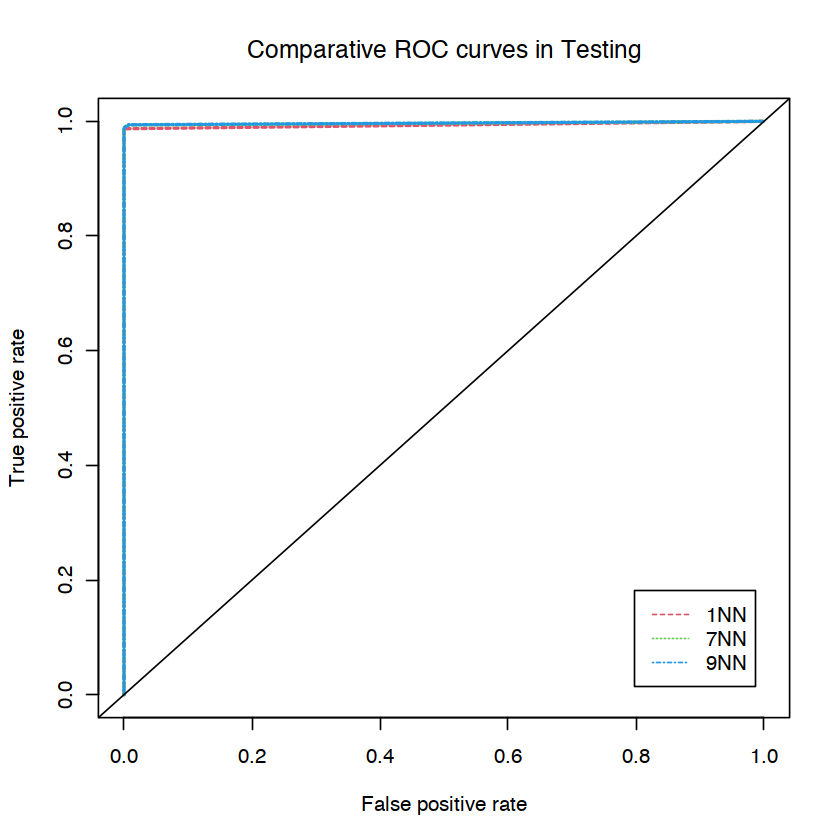
\includegraphics[width=330pt,  height=170pt]{./graphics/q32.png}
			\caption{Comparative ROC Curves in Testing}
		\end{figure}
	\item[(3)] Solution in the r file
	\item[(4)]  From the ROC Curve, it is clear that 1NN has the highest model complexity whilst 7NN has the 
 least model complexity. Therefore, according to Ocam's Razor, the model with the least complexity 
must be preferred.
\item[(5)] Solution in r file
\end{enumerate}
\section*{Exercise Bonus 1}
The point-wise bias variance decomposition
when $\hat{f}$ is the k Nearest Neighbors regression learner.

Let  $\mathscr{D}_n :=\lbrace{(\mathrm{x}_i,yi) \overset{\text{iid}}{\sim} p_{\mathrm{x},y}(\mathrm{x},y) ,  \mathrm{x}_i \in \mathbb{R}, y_i \in \mathbb{R}\rbrace_{ i= 1}^n}.$ 
\begin{align*}
\widehat{f}_{kNN}(x)  &= \frac{1}{k} \sum_{i=1}^{n} y_i \mathbb{1}(x_i \in V_k(x))\\
\end{align*}
where 
\begin{align*}
   V_k(x) := \{  x_i \in \mathscr{D}_n   \quad  \text{ s.t.   }  d(x,x_j) \leq d(k) \}
\end{align*}
where $d(k)$ being the shortest $k$-th distance from the new data-point  $x$.

Thus, for the variance of $ \widehat{f}_{kNN}$:
\begin{align*}
  \text{Variance} \left(  \widehat{f}_{kNN}(x)\right) &=  \mathbb{V}(\frac{1}{k}  \sum_{i=1}^n y_i \mathbb{1}(x_i \in V_k(x))\\
  &=  \frac{1}{k^2}  \sum_{i=1}^n \mathbb{V}[y_i | x_i] \mathbb{1}(x_i \in V_k(x))\\
  &= \frac{1}{k^2}  \sum_{i=1}^n \sigma^2 \mathbb{1}(x_i \in V_k(x))\\
  &= \frac{k\sigma^2}{k^2} \\
  &= \frac{\sigma^2}{k}
\end{align*}
For the bias of $ \widehat{f}_{kNN}$:
\begin{align*}
  \text{Bias} \left(  \widehat{f}_{kNN}(x)\right) &=  \mathbb{E}[ \widehat{f}_{kNN}(x)]  - f(x)\\
  &=  \frac{1}{k}  \sum_{i=1}^n y_i \mathbb{1}(x_i \in V_k(x)) -  f(x)\\
  &= \frac{1}{k}  \sum_{i=1}^n \mathbb{E}[y_i | x_i] \mathbb{1}(x_i \in V_k(x)) -  f(x)
\end{align*}
Given that 
\begin{align*}
		 \mathbb{E}[y_i | x_i]  &= (fx_i)
\end{align*}
Therefore 
\begin{align*}
	  \text{Bias} \left(  \widehat{f}_{kNN}(x)\right) &=   \frac{1}{k}  \sum_{i=1}^n f(x_i)  \mathbb{1}(x_i \in V_k(x)) -  f(x)\\
	  &=   \frac{1}{k}  \sum_{x_i \in V_k(x)} f(x_i) - f(x)
\end{align*}
Finally, the point wise decomposition of $\text{MSE}\left(  \widehat{f}_{kNN}(x)\right) $ is:
\begin{align*}
	\text{MSE}\left(  \widehat{f}_{kNN}(x)\right) &= \sigma^2 + \frac{\sigma^2}{ k} + \left(     \frac{1}{k}  \sum_{x_i \in V_k(x)} f(x_i) - f(x)   \right)^2
\end{align*}
\section*{Exercise Bonus 2}
Solution in the r file.
\end{document}